\subsubsection{Completed Strict L-only Readouts}

The six reuse-only readouts are complete: F15 and F20 each provide three corrected F seeds, paired with the same F0 G-L whose eight training ancestors use labeled-source IQ only. Each row freezes raw and restored predictions for all seven views before independent truth-last scoring. The target contract remains seven receivers and 168000 packets per view.

\begin{table}[t]

\centering\scriptsize

\caption{Strict L-only F0 accuracy (\%, mean$\pm$sample SD over three F seeds conditional on one fixed G-L).}

\label{tab:Lonly6}

\setlength{\tabcolsep}{2pt}

\begin{tabular}{llrrr}

\toprule

F recipe & Readout & Clean & Six views & Low urban \\

\midrule

X3\_CE & raw & $81.5486\pm1.3443$ & $46.3480\pm1.7442$ & $34.9881\pm0.7976$ \\

X3\_CE & DURA-L & $81.4298\pm1.3283$ & $74.4888\pm1.1408$ & $63.5004\pm1.0796$ \\

T1\_SUP & raw & $84.7853\pm0.8236$ & $70.5962\pm0.9519$ & $51.6397\pm0.5500$ \\

T1\_SUP & DURA-L & $84.7679\pm0.8511$ & $76.8537\pm0.5918$ & $65.7323\pm0.2781$ \\

\bottomrule

\end{tabular}

\end{table}

F15 uses ordinary-view CE plus default satellite-concatenation CE (weight 0.68), with zero label smoothing and no CRIC, paired KL, U or EMA. F20 retains the supervised T1 CRIC, ordinary/raw KL, As CE with As KL zero, and label smoothing 0.01, while disabling U and EMA. Their 50 logical epochs and 11100 updates match, but actual labeled-packet forward evaluations are 384 versus 768 per update and the augmentations differ. The contrast therefore compares complete supervised recipes, rather than identifying one component effect or replacing the matched CE structural controls.

G-L improves the six-view means by $+28.1408\pm1.3019$ and $+6.2575\pm0.3641$ percentage points for F15 and F20, respectively. The paired clean changes are $-0.1188\pm0.0274$ and $-0.0175\pm0.0501$ points; these small negative means are retained. Six-view averaging precedes seed-paired differences and sample SD; the latter is not a significance test.

\begin{figure*}[t]

\centering

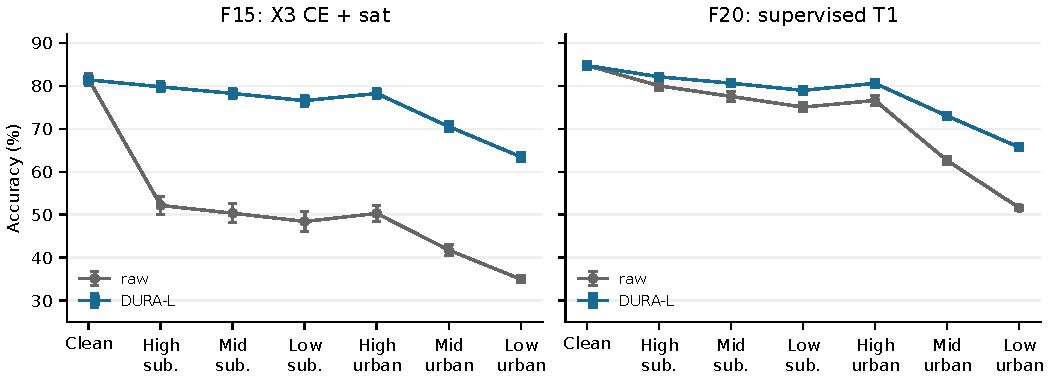
\includegraphics[width=\textwidth]{images/Lonly6/Lonly_seven_views.pdf}

\caption{Completed raw and G-L readouts on all seven F0 views. Error bars are three-F-seed sample SD conditional on the same labeled-only restorer. Every negative clean change is retained; these curves do not select a replacement recipe.}

\label{fig:Lonly6}

\end{figure*}

All 4032 serialized confusion matrices, 2016 stratum-level correction nets, and exact reuse of same-F raw matrices were checked. The six source-physics panels each reuse the same 720 labeled packets across 90 TX/RX/day strata and 11 interventions, with no U, target access, or fitted probe. They characterize sensitivity and inductive bias, not complete hardware disentanglement or identity preservation under synthetic PA changes.

No additional F or G was trained for these readouts. The reused six F trajectories total 6.836 shared-worker hours, and the one reused eight-stage G-L totals 4.826 hours; these are historical elapsed costs, not incremental or exclusive GPU time. The separate 24-model architecture panel and its dedicated online timing remain incomplete.
